% arara: lualatex: { shell: yes }
% arara: lualatex: { shell: yes }
% arara: clean: { files: [ moab.aux, moab.dvi, moab.log, moab.out, moab.out.ps ] }
% arara: clean: { files: [ moab.toc, moab.idx, moab.ind ] }

\documentclass[12pt]{scrartcl}
	\usepackage[automark,headsepline]{scrpage2}
	\usepackage[english]{babel}
	\usepackage[hidelinks]{hyperref}
	\usepackage{bookmark}
	\usepackage{titlesec}
	\usepackage{lastpage}
	\usepackage{footmisc}
	\usepackage{ifxetex,ifluatex}
	\usepackage[T1]{fontenc}
	\ifluatex\usepackage{luatextra}\fi
	\usepackage{libertine}
	\usepackage{microtype}
	\usepackage[xindy]{imakeidx}
	\usepackage{verbatim}
	\usepackage{varioref}
	\usepackage{environ}
	\usepackage{listings}
	\usepackage{wrapfig}
	\usepackage{graphicx}
	\usepackage{fancybox}

	\makeatletter

	\AtBeginDocument{
		\hypersetup{
			pdftitle = {\@title},
			pdfauthor = {\@author}
		}
		\pagestyle{scrheadings}
		\ihead{\MakeUppercase{\@title}}
		\chead{}
		\ohead{\leftmark}
		\ifoot{}
		\cfoot{Page \pagemark{} of \pageref{LastPage}}
		\ofoot{}
	}

	% hack to get title macro back after \maketitle clears it
	% see http://tex.stackexchange.com/a/164232/5100
	\let\svmaketitle\maketitle
	\def\maketitle{\protected@edef\saved@title{\@title}%
	\svmaketitle%
	\let\@title\saved@title}%

	% Use OTF fonts from the Libertine project across the board
	\defaultfontfeatures{Ligatures=TeX}
	\setmainfont{Linux Libertine O}
	\setsansfont{Linux Biolinum O}
	\setmonofont{Linux Libertine Mono O}

	% Instanciate our main document index and tell texindy how to format it
	\makeindex[intoc,columns=2]

	% Set default values for formatting verbatim examples
	\def\lstlistlistingname{List of examples}
	\lstnewenvironment{ExampleCode}[1][snippet.tex]{%
		\def\lstlistingname{Example}
		\lstset{%
			float=here,
			language=tex,
			numbers=left,
			numberstyle=\tiny,
			xleftmargin=2em,
			xrightmargin=2em,
			frame=l,
			framesep=1ex,
			caption=[snippet: #1]~,
			label=#1
		}
		\ttfamily
	}{}
	\lstnewenvironment{ExampleFile}[1][example.tex]{%
		\def\lstlistingname{Example}
		\lstset{%
			language=tex,
			numbers=left,
			numberstyle=\tiny,
			xleftmargin=2em,
			xrightmargin=2em,
			frame=shadowbox,
			framesep=1ex,
			title=#1,
			caption=[file: #1]#1,
			label=#1
		}
		\ttfamily
	}{}

	% Don't let footnotes wrap to following pages
	\interfootnotelinepenalty=5000

	% Get the bibliography, TOC etc. to show in the TOC
	\usepackage{tocbibind}

	% Set the bibliography title
	\renewcaptionname{english}{\refname}{References and Credits}

	% Format section titles to the right more like chapters
	\newcommand{\sectionbreak}{\clearpage}
	\titleformat{\section}
		{\sffamily\Large\bfseries\raggedleft}
		{\thesection}
		{2\wordsep}
		{}

	\setlength{\shadowsize}{2pt}

	% So impressive can read our output
	\pdfminorversion=4
	\makeatother

\title{Memoirs of a Bulletin}
\subtitle{The Voice of One Making Straight the Way for Well-Typeset Liturgies}
\author{Caleb Maclennan}

\begin{document}

\pagenumbering{roman}

\maketitle

\vfill

\begin{abstract}

As long as today is still called ``today''\footnote{Hebrews 3:13}, Sunday will
keep coming every Sunday~\dots~but typesetting the bulletin every week doesn't
have to be a chore\footnote{Leviticus 23:3}---nor do the results have to be an
eyesore! Even for people like myself who are not graphically inclined, there are
ways to make the process of producing well-typeset documents a relatively
painless process.

While the \emph{resulting} system may be relatively painless to use, discovering
these systems, learning the necessary techniques and applying them to the
process of producing bulletins is not so easy the first time around. I write
this article to document my own findings in hopes that it will make the same
journey easier for any that would follow.

\end{abstract}

\section*{Prologue}
\addcontentsline{toc}{section}{Prologue}

The pastor of my church has many great strengths. He has sound theology and,
shall we say, an appreciation for both the Word in partucular and printed words
in general. Yet for all his immense love of books, he does not really understand
typography or the art of what transforms raw text into effective communication.
His version of 'typesetting' is to underline everything, then bold a few
important bits that got lost in the lines.\footnote{To his credit, I've seen
	much worse. While his choice of formatting combinations isn't always
	well advised, he does refrain from heinous crimes like using five
	different typefaces on a single page.} Our church does not have the
discinction of having a secretary.\footnote{Volunteers welcome! Brush up on your
	Turkish and I'll put you to work.} That leaves me---a programmer not a
designer---typesetting most of the material we produce. While this is less than
ideal, I have found there are tools that make the work easier and keep me out of
too much trouble.

When I started down the road of typesetting our bulletins using \LaTeX, I was
unable to find much helpful documentation out there. \LaTeX itself is
extensively documented, but few of the examples available are applicable to the
special needs of bulletins. The system excels at books and articles, but needs
some extra love to produce smaller scale work with more formatting than content.
I did find a few others online that had traveled the road before me. Some of
these will be credited in this text, but others will rename nameless for fear of
this reading like a hall of shame. Yes, some of them were that bad.\footnote{One
	entry went so far as to align footers on each page by inserting empty
	boxes in the body after the page content with hard coded heights that
	had been carefully measured to push the remaining content to roughly the
	bottom of each page!}. Most samples wanted te end up with a booklet
format, but the way they arrived at the desired output was not semantic and
cumbersome at best.\footnote{Having that special service where your liturgy runs
	over your usual page length shouldn't destroy your publishing process;
	nor should you have to remember that pages 1, 2, 3, and 4 of your
	printed bulletin are actually saved in your source as 4, 1, 2, and 3
	respectively.}

In the following pages I will outline the methods I came up with and the lessons
I learned. The system I came up with will not work for all churches. In many
cases your needs may be simpler. Some of you may have more complex requirements.
In one sense a church bulletin is nothing more than a priece of paper with a few
words outlining a service to keep everybody on the same page. Yet it is a kind
of `tell': the contents, layout and usage of a church's bulletin can tell you a
lot about the church because it reflects in large part their theology of
worship. You will find a good deal of my own theology in the following pages and
some of the techniques will be more or less useful to you depending on your
church's understanding of liturgy. I will make no apology for my own theology;
how you adapt this is your business. I present my system not expecting it to be
a drop in solution, but in the hopes that at least some of the pieces may be
adaptable to other church's needs.

\tableofcontents

\pagenumbering{arabic}

\section{Why not just use a word processor?}

\index{Word}
Why Microsoft Word is not the tool for the job.

\index{LibreOffice}
My weapon of choice would be LibreOffice, but this didn't get me much further.

Why alternatives like page layout programs don't quite cut the mustard.

Bad bad typography.

If you think the example on the left is better that the right, stop reading now
and walk away.

(bad example figure) (good example figure)

Special events shouldn't require starting from scratch with a totally new
layout. Memorial services, weddings, seminars, etc should be easily adaptable
from existing publishing workflow.

You shouldn't be copy-pasting a bunch of repetitive parts or trying to remember
what week you used that special thing...

\section{What is the right tool for the job?}

Have more than a hammer.

Use real typesetting tools.

\index{InDesign}\index{Quark Express}
InDesign, Quark

\index{Linux}
Most are not free, not portable, won't run on Linux, produce output that is not
maintainable.

\subsection{Why \LaTeX?}

Simple. Versatile. Accurate. Readable. Consistent.

Portable output. (booklet, full page, pdf, ebook, web)

\subsubsection{But won't \LaTeX be bad for my health?}

There are a couple pitfalls to be aware of.

\subparagraph{Your congregation might get the wrong idea.}

When they hear you are using something called 'latex' and plug that search term
into Google all by itself, it's probable that what comes up first will be NSW
and certainly not safe for the church office. It's unfortunate that the name
should be hijacked by a fetish, but once you start searching for \texttt{latex +
	<anything document related>} the problem pretty much goes away.

\subparagraph{You can't set this up on a Sunday morning.}

The initial setup is a little complicated to setup. You can't do this at the
last minute, you will need to prepare your system in advance. Do this on a week
where you have some extra time and think about how to handle you special
services \emph{before} they happen rather that when you are already swamped
getting ready for them.

Your secretary might actually \emph{never} end up like it. Good semantic
document structure is inherently limiting. This can be a good thing, but it will
feel like a loss of freedom to some.\footnote{Gratuitous parallel to how freedom
	in Christ is limiting to our lifestyle but the result being for our
	good.}

\subsection{Are there other alternatives?}

There really aren't other viable alternatives in this class. Unless you want to
hand code generating PDF's from code of your own\footnote{This is actually not
	\emph{that} hard to do and is what I started to do before realizing that
	\LaTeX was a better tool for the job. The disadvantage is that tweaking
	your layout to match your ever changing content is complex and not
	something the church secretary is going to pull off. Good typesetting
	rather that just filling in a few blanks quickly gets too cumbersome and
	I gave up this route.} Your only other choice is to use a page layout
tool. Quark Express used to be the old standby for church use, but InDesign is
the popular kid on the block in this space today.

\section{Where do I start?}

\subsection{How do I install the tools?}
\label{sec:install}

See also installing git in section~\vref{sec:gitinstall}

\subsubsection{TeX distributions}

texlive, mactex, <windows>?

\subsubsection{TeX editors}

gedit, texmaker, vim, emacs, notepad++, etc

\subsection{lilypond}

\subsection{Picking a complier}
\label{sec:compiler}

\index{PdfTeX}\index{LuaTeX}\index{XeTeX}

Should you use pdftex, luatex, xetex?

Recommend luatex...

\subsection{How do I make it do something?}

\begin{ExampleFile}[helloworld.tex]
\documentclass{letter}
\begin{document}
Hello world!
\end{document}
\end{ExampleFile}

See example~\vref{helloworld.tex}

\subsection{How do I use the examples in this tutorial?}

All the sample files and tools mentioned in this tutorial are available at
Github\footnote{\url{https://github.com/alerque/moab}}. You may browse and download them
individually from there, but there is a better way.

Clone the whole repo...

Once you have a cloned copy of the repository, all the examples should be
available in the ./examples folder. They may be compiledd using most any latex
complier. See section~\vref{sec:compiler} for help picking one.

Or if you would like to contribute your changes back to this project, start by
using the "Fork" link at the top right of the Github page.

\section{What is the essence of a bulletin?}

We covered this already in example~\vref{helloworld.tex}.

In which I rant against church services being about entertainment.

The bulletin should be useful but not take front stage. It should be readable,
communicate it's message and get out of the way.

\subsection{Rounding up the usual suspects}

Think carefully about what you may need to include, consider \emph{not}
including some things you might normally think of as par-for-the-course.

Church info

announcements

\subsection{Liturgical styles}

What you include may vary and have unique formatting requirements.

Responsive readings.

Creeds.

\subsection{Coordinating other media types}

Interfacing with content used elsewhere (web, projection, mobile)

\subsubsection{Beamer}

\index{Beamer}
Because its cool.

\subsubsection{Impressive}
\index{Impressive}
Because it's pretty and it reads from Beamer like a dream.

\section{All the things you can do}

\subsection{Headers and footers}

Using the sparingly, they will make printing different layouts harder.

fancyhdr vs scrpage2

\subsection{Debugging your layout}

\index{Debuging}
Figuring out \emph{why} something is the way it is in a rendered \LaTeX~document
is not that easy, but there are a few tricks you can use.

\index{\verb+\usepackage{showframe}+}
As you begin your initial layout and are trying to understand the basic page
formatting  rules, it can be helpful to see where the page margigns are. You can
de this by enabling the \texttt{showframe} package as in
example~\vref{showframe}.

\begin{wrapfigure}[5]{r}{0.5\textwidth}
	test
\end{wrapfigure}

\begin{ExampleCode}[showframe]
\usepackage{showframe}
\end{ExampleCode}

\section{Putting it all together}

Bring alll the bits from the previous section

\subsection{A working template}

%\verbatiminput{/home/caleb/projects/ipk_belgeler/toplanti/deneme.tex}

\subsection{Beam me up Scotty! (compile time considerations)}

Why multi-pass is necessary.

\index{Arara}
Arara.

\section{But how do I print it?}

Not by reaching for File » Print from your text editor!

You generate finished documents (usually in PDF format).

\subsection{Booklet printing}
\index{Booklet}

\subsubsection{The easy way with pdf}

\section{How do I organize all this stuff?}

Whether alone or not, managing files that collect over time...

\subsection{The hard way(s)}

\subsection{The right way: version control}

\subsubsection{VCS Systems}

\index{VCS}\index{DVCS}\index{Subversion}

Distributed vs dumb.

\subsection{GIT magic}
\index{Git}

\subsubsection{Installing Git}
\label{sec:gitinstall}

\subsubsection{Using git to organize bulletin files}

In which the use of \texttt{git} is explained in relation to Bulletin
management.

\begin{verbatim}
# git init
\end{verbatim}

\section{Advanced wizardry}

\subsection{A better tomorrow, made possible by macros}
\index{Macros}

How to write custom commands for oft-repeated tasks.

\subsection{Using external files}


\subsubsection{Sourcing liturgical bits}

Keeping your creeds, responsive readings, etc. in separate files.

Including other content such as sermon outlines that is also published
separately.

\subsubsection{Backfill}

\index{Backfill}

This is tricky from paul \cite{backfill}

\subsubsection{Pulling data from external API's}

Auto importing verse data from the web.

\subsection{Is that a song I hear?}
\index{Music}

Why including music in the bulletin can be good for worship.

\subsubsection{Lilypond to the rescue}
\index{Lilypond}

\subsection{Language considerations}
\index{Language}

Every tongue.

\subsubsection{Using different encodings}

\subsubsection{Multi-lingual output}

Examples of parallel typeset content in two languages.

Or make two print editions with different content from the same source.

\subsection{Preparing for multiple services}

Using the same bulletin source with if-statements to output only relevant
content for each service.

\subsection{Multiple print editions}
\index{Arara}

Have your cake and eat it too. Or, 'the two bulletin church' rather that the
'two service church'.

\section{Out-takes}

Because more sections are good right?

\subsection{Gallery}

Some inspiring examples of well typeset bulletins!

\begin{figure}[h]
	\centering
	\begin{tabular}{@{}c@{\hspace{1em}}c@{}}
		\shadowbox{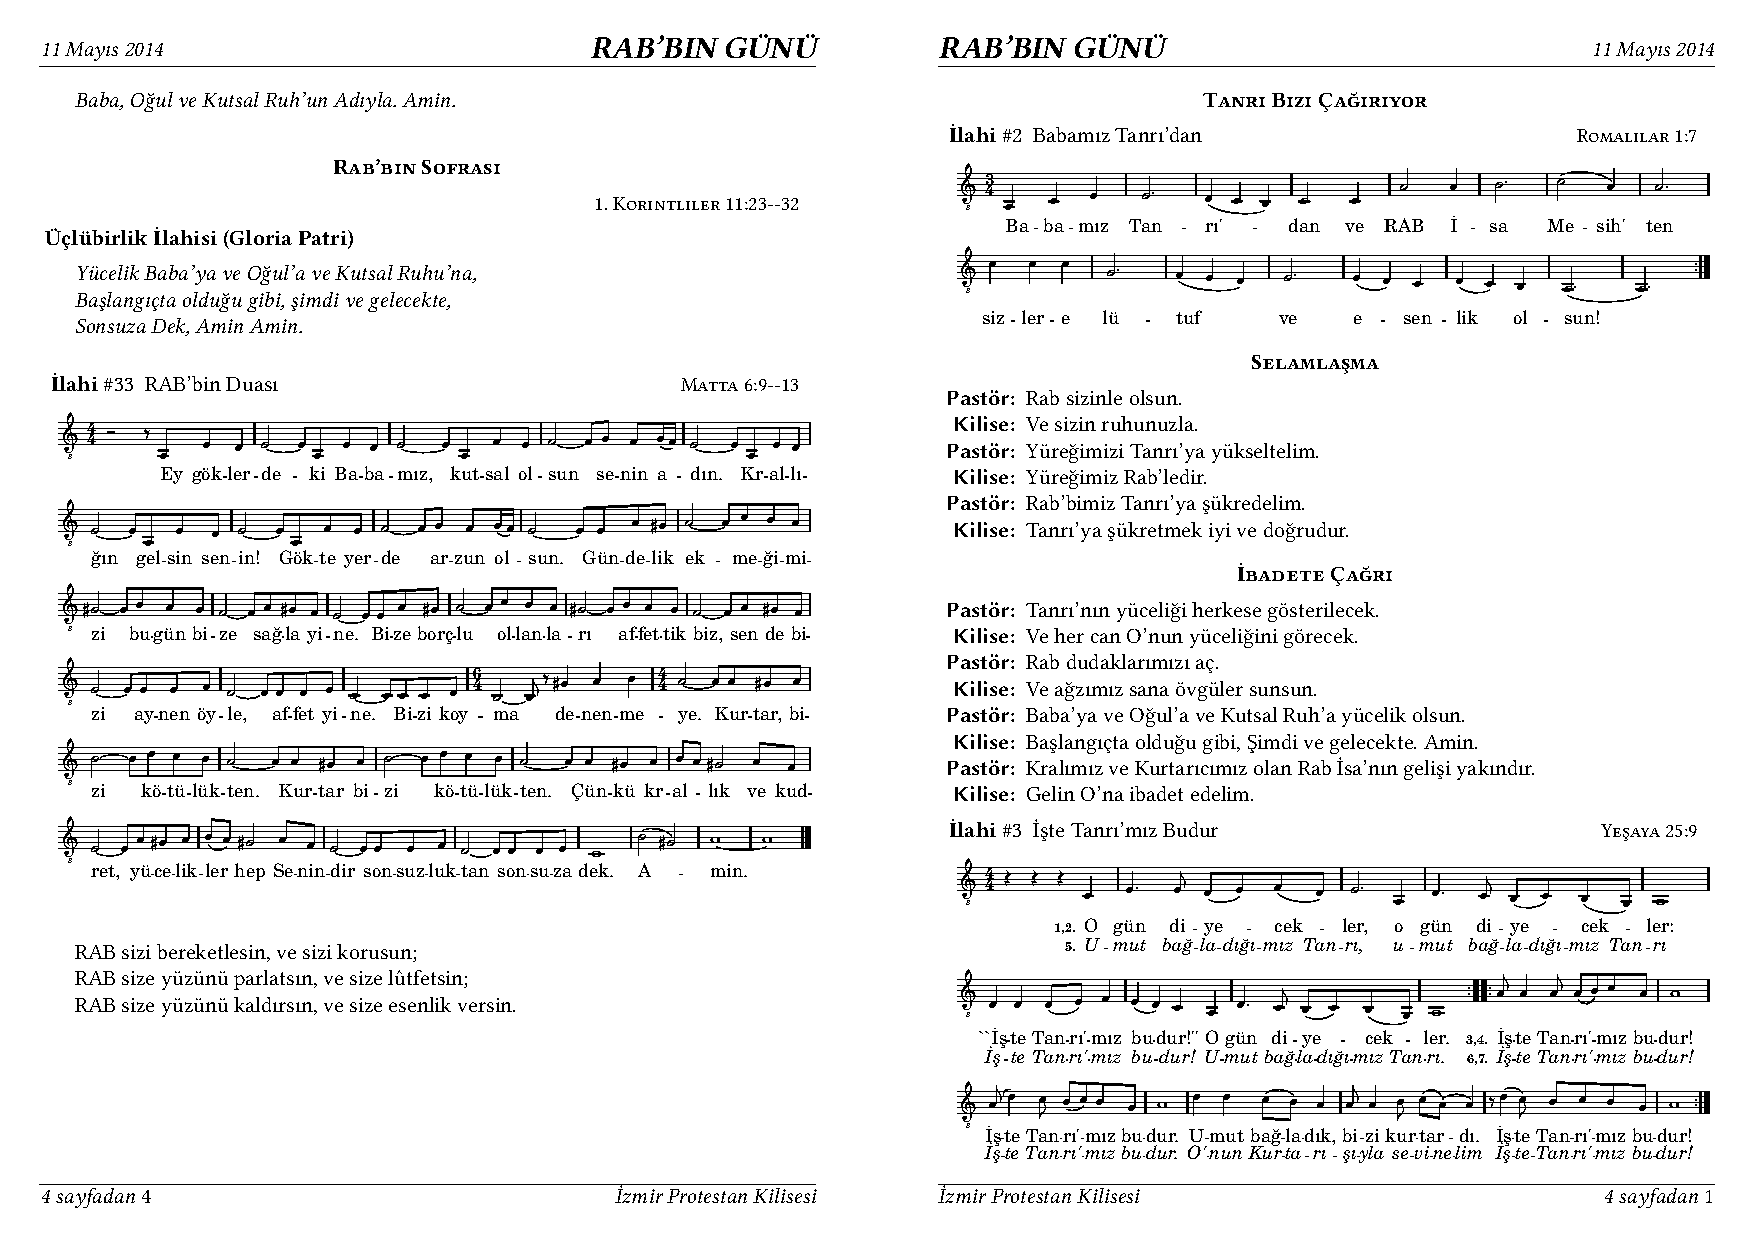
\includegraphics[page=1,width=.9\textwidth]{../gallery/ipk.pdf}} \\[1ex]
		\shadowbox{\includegraphics[page=2,width=.9\textwidth]{../gallery/ipk.pdf}}
	\end{tabular}
	\caption{The Protestant Church of Smyrna}
	\label{ipk}
\end{figure}

\begin{figure}[h]
	\centering
	\begin{tabular}{@{}c@{\hspace{1em}}c@{}}
		\shadowbox{\includegraphics[page=1,width=.45\textwidth]{../pub/moab.pdf}} &
		\shadowbox{\includegraphics[page=2,width=.45\textwidth]{../pub/moab.pdf}}
	\end{tabular}
	\caption{This document}
	\label{self}
\end{figure}

\begin{thebibliography}{99}
	\bibitem{tex.se}
	Tex Stack Exchange:\\
	\url{http://tex.stackexchange.com}
	\bibitem{backfill}
	Thanks to Paul Stanley and his answer to my question:\\
	\url{http://tex.stackexchange.com/q/174028/5100}
\end{thebibliography}

\printindex

\clearpage
\addcontentsline{toc}{section}{\lstlistlistingname}
\lstlistoflistings

\end{document}
% vim: textwidth=80
